%%%%%%%%%%%%%%%%%%%%%%%%%%%%%%%%%%%%%%%%%%%%%%%%%%%%%%%%%%%%%%%%%%%%%%%%%%%%
%% Trim Size: 9.75in x 6.5in
%% Text Area: 8in (include Runningheads) x 5in
%% ws-mpla.tex   :   29-9-2008
%% TeX file to use with ws-mpla.cls written in Latex2E.
%% The content, structure, format and layout of this style file is the
%% property of World Scientific Publishing Co. Pte. Ltd.
%% Copyright 1995, 2002 by World Scientific Publishing Co.
%% All rights are reserved.
%%%%%%%%%%%%%%%%%%%%%%%%%%%%%%%%%%%%%%%%%%%%%%%%%%%%%%%%%%%%%%%%%%%%%%%%%%%%
%%

\documentclass{ws-mpla}
\usepackage[super]{cite}
\usepackage{graphicx}
\begin{document}

\markboth{Authors' Names}{Instructions for Typing Manuscripts (Paper's Title)}

%%%%%%%%%%%%%%%%%%%%% Publisher's Area please ignore %%%%%%%%%%%%%%
\catchline{}{}{}{}{}
%%%%%%%%%%%%%%%%%%%%%%%%%%%%%%%%%%%%%%%%%%%%%%%%%%%%%%%%%%%%%%%%%%%

\title{IMPLEMENTATION OF THE XXXXX-XXXX-XXXX-XX ANALYSIS IN THE MADANALYSIS 5 FRAMEWORK}

\author{\footnotesize FIRST AUTHOR}
\address{
  University Department, University Name, Address\\
  City, State ZIP/Zone, Country}

\author{SECOND AUTHOR}
\address{
  University Department, University Name, Address\\
  City, State ZIP/Zone, Country}

\maketitle

\pub{Received (Day Month Year)}{Revised (Day Month Year)}

\begin{abstract}
We present the MADANALYSIS 5 implementation and validation of the
XXXXX-XXXX-XXXX-XX search (give the search identifier: CMS-EXO-17-013, etc...).
Then describe in one sentence the targeted signature, the luminonsity of
analysed data. Explain also in one sentence how the validation was performed.
If a short physics is performed during the school, please mention it as well.
\keywords{Keyword1; keyword2; keyword3.}
\end{abstract}

%\ccode{PACS Nos.: include PACS Nos.}

\section{Introduction}
Here, present briefly the classes of new physics signals investigated in the LHC
analysis and describe the signature relevant for the search. Detail the model on
which the validation is based on, as well as the benchmark (how the model
parameters have been fixed) and the signal.

\section{Description of the analysis}
Describe in one or two sentences the main idea behind the event selection
strategy.

\subsection{Object definitions}
Detail here all the objects that are used in the analysis. This should include
typical selection cuts like $p_T$ and $|\eta|$ requirements, isolation criteria,
jet definitions, {\it etc.} Please ignore stuff that we cannot simulate in our
machinery.

\subsection{Event selection}
Detail here the different cuts and how they define the different signal regions.
A table may be useful to show everything in a compact way.

\begin{table}[t]
  \tbl{Please use this template for tables.}
  {\begin{tabular}{@{}cccc@{}} \toprule
  Piston mass & Analytical frequency & TRIA6-$S_1$ model &
  \% Error \\
  & (Rad/s) & (Rad/s) \\
  \colrule
  1.0\hphantom{00} & \hphantom{0}281.0 & \hphantom{0}280.81 & 0.07 \\
  0.1\hphantom{00} & \hphantom{0}876.0 & \hphantom{0}875.74 & 0.03 \\
  0.01\hphantom{0} & 2441.0 & 2441.0\hphantom{0} & 0.0\hphantom{0} \\
  0.001 & 4130.0 & 4129.3\hphantom{0} & 0.16\\ \botrule
  \end{tabular}\label{ta1} }
\end{table}


\section{Validation}

\subsection{Event generation}

Give information on how the event samples relevant for the validation of the
analysis have been generated. Provide details about the generators that have
been used, their versions, the model files, etc.

\subsection{Comparison with the official results}
In this section, you should put all the comparisons you have made. Cutflows in
which you compare the MA5 numbers to the official ATLAS/CMS ones, distributions
if any. Put here as much material as possible. Of course this depends on the
pieces of information available in the analysis. Assess the level of agreement,
why you think it is correct, etc.

\begin{figure}[t]
  \centerline{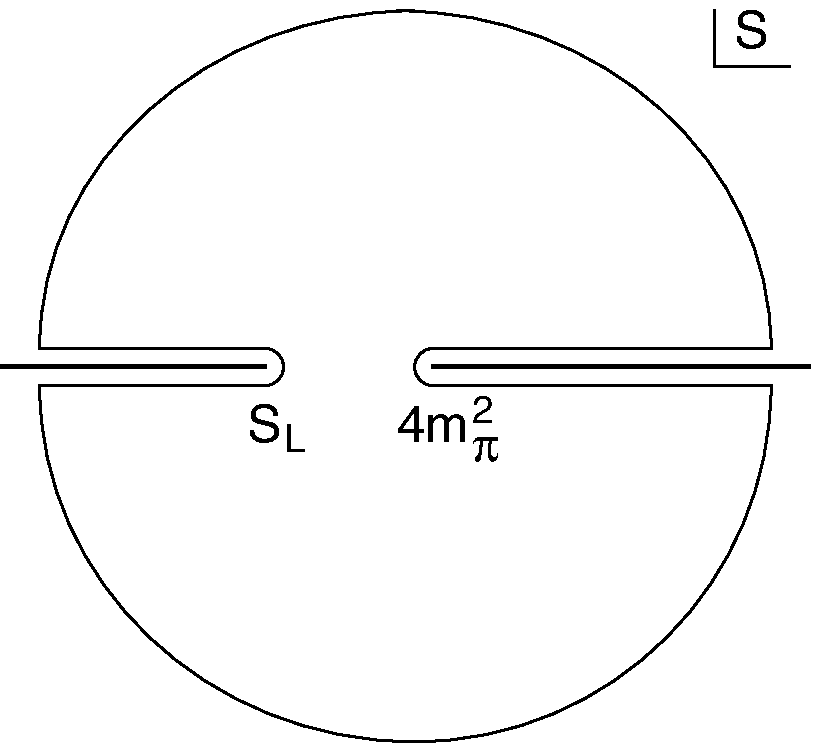
\includegraphics[width=2.0in]{mplaf1}}
  \vspace*{8pt}
  \caption{Please use this template for figures.\protect\label{fig1}}
\end{figure}

\section{Conclusions}
Summarise your work here.

\section*{Acknowledgments}
Dedications and funding information may be included here.

\begin{thebibliography}{0}
\bibitem{Conte:2018vmg}
  E.~Conte and B.~Fuks,
  Int.\ J.\ Mod.\ Phys.\ A {\bf 33} (2018) no.28,  1830027
  [arXiv:1808.00480 [hep-ph]].

\bibitem{Dumont:2014tja}
  B.~Dumont {\it et al.},
  Eur.\ Phys.\ J.\ C {\bf 75} (2015) no.2,  56
  [arXiv:1407.3278 [hep-ph]].

\bibitem{Conte:2014zja}
  E.~Conte, B.~Dumont, B.~Fuks and C.~Wymant,
  Eur.\ Phys.\ J.\ C {\bf 74} (2014) no.10,  3103
  [arXiv:1405.3982 [hep-ph]].

\bibitem{Conte:2012fm}
  E.~Conte, B.~Fuks and G.~Serret,
  Comput.\ Phys.\ Commun.\  {\bf 184} (2013) 222
  [arXiv:1206.1599 [hep-ph]].

\end{thebibliography}
\end{document}
